\documentclass[11pt]{article}
\usepackage[romanian]{babel}
\usepackage[utf8]{inputenc}
\usepackage[T1]{fontenc}
\usepackage{amsmath}
\usepackage{amsfonts}
\usepackage{amssymb}
\usepackage[version=4]{mhchem}
\usepackage{stmaryrd}
\usepackage{graphicx}
\usepackage[export]{adjustbox}
\graphicspath{ {./images/} }

\begin{document}
Private Equity Funds of Funds Historical Returns

\section*{Key Observations Regarding Historical Returns of PE Fund of Funds}
Given the diversification benefits, and the expertise of PE FoFs, how well do they perform net of their double layer of fees? There are few reports on the performance of PE FoFs, and even fewer on the benchmarking of PE FoFs. ${ }^{1}$ Burgiss, Preqin, and ILPA are some industry sources that track the return performance of PE FoFs, but there are few benchmarking reports publicly available. Gresch and von Wyss (2011) compared PE FoFs to investments in single PE funds. Using IRR and multiples of invested capital, they concluded that PE FoFs have lower return dispersion than investing in single PE funds in the same vintage year. Return dispersion describes the possible range of returns for an investment. A higher return dispersion implies there a wider range of potential returns, measuring an increased risk of the investment. Harris, Jenkinson, Kaplan, and Stucke (2015) benchmarked PE FoFs to public equity market performance using Kaplan-Schoar PME (KS-PME). KS-PME is a ratio that compares private equity performance relative to the public market index. A KS-PME of greater than 1 implies outperformance relative to the public market benchmark. As shown in the next exhibit, PE FoFs have an average KS-PME ratio of 1.13; thus, on average, PE FoFs provide returns above public equity market performance. They also benchmarked PE FoFs to portfolios of PE funds as opposed to single PE funds since FoFs are invested across PE funds; thus, comparing a portfolio would better match PE FoFs. The exhibit shows that PE FoFs have an average KS-PME of 1.13, while a portfolio of PE funds has an average KS-PME of 1.19. While PE FoF outperform public market equity investments, they do not outperform portfolios of direct investments in PE funds.

\begin{center}
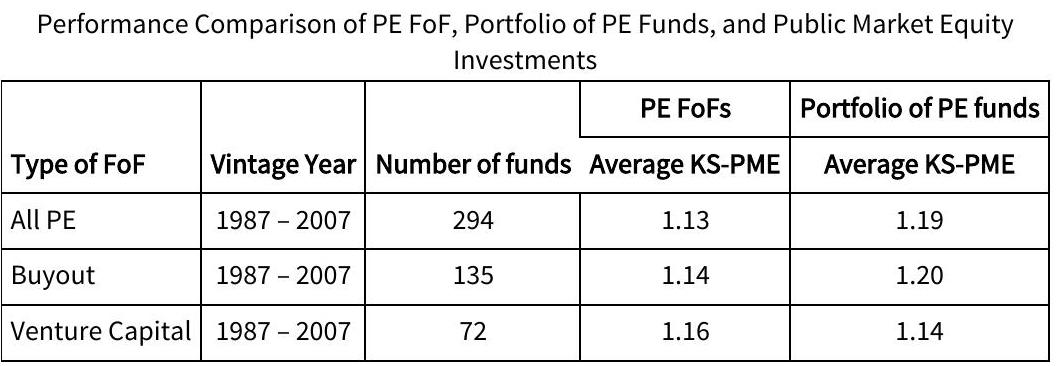
\includegraphics[max width=\textwidth]{2024_04_10_9f7c3d00b4613a650b6cg-2}
\end{center}

Source: CAIA Association. Data from Harris, Jenkinson, Kaplan, and Stucke (2015).

The results of these studies suggest the following. First, PE FoFs do offer diversification benefits by reducing performance dispersion. Second, overall PE FoFs do provide higher return than investing in public equity markets, but at the cost of higher illiquidity. Third, PE FoFs returns are lower than a portfolio of PE funds. This could be due to the double layer of fees. The portfolio of PE funds assumes that an investor has no limitation in selecting the PE funds, but access to some PE funds may be limited for some investors because of oversubscription and the challenge of identifying top PE funds.

\section*{Buyout Fund of Funds versus Its equivalent Portfolio of Funds}
As shown in earlier sections, private equity can be further divided into three broad categories-venture capital, growth equity, and buyout. Buyout is at the lower end of the risk spectrum, while venture capital is at the higher end of the risk spectrum. PE FoFs can also be further categorized. Harris, Jenkinson, Kaplan and Stucke (2015) used the fund of funds categories in Burgiss database and created similar portfolios of PE funds. ${ }^{2}$ Burgiss categorizes funds of funds as 1 ) corporate finance, 2 ) generalist, or 3) venture capital. Corporate finance category largely targets buyout funds. The generalist category has a mixed of corporate finance and venture capital. Venture capital category solely focuses on venture capital. They benchmarked whether buyout FoFs performed better than a portfolio of buyout funds. They concluded the following:

\begin{itemize}
  \item Buyout FoFs have smaller dispersion in performance than single buyout funds. The standard deviation of KS-PMEs against the S\&P 500 is reduced to about half the comparable value for buyout funds. This is the result of diversifying across funds and vintage years.
  \item Buyout FoFs have lower return against a similar portfolio of funds. This is shown in the exhibit Performance Comparison of PE FoF, Portfolio of PE Funds, and Public Market Equity Investments, where the buyout FoFs have an average KS-PME ratio of 1.14 while portfolio of buyout funds have an average KS-PME ratio of $1.20 \mathrm{implying}$ buyout FoFs underperform relative to its equivalent portfolio of funds. This suggests an investor could be better off creating a portfolio of PE funds if they exhibit fund selection skills and have access to top-performing managers.
\end{itemize}

\section*{Venture Capital Fund of Funds versus Its Equivalent Portfolio of Funds}
Harris, Jenkinson, Kaplan, and Stucke (2015) also benchmarked whether venture capital funds of funds (VC FoFs) performed better than its equivalent portfolio of venture capital funds (VC funds). They concluded the following:

\begin{itemize}
  \item VC FoFs have smaller performance dispersion than single VC funds. The standard deviation of KS-PMEs against the S\&P500 is reduced to about one-third the comparable value for single VC funds. In addition, the reduction in performance dispersion is greater than that of buyout FoFs. This suggests that the diversification benefit delivered by funds of funds depends on the underlying variability in fund performance. The greater the underlying variability in fund performance, the greater the diversification benefit delivered by the fund of funds.
  \item VC FoFs performed on par against a portfolio of VC funds. This is shown in the exhibit Performance Comparison of PE FoF, Portfolio of PE Funds, and Public Market Equity Investments, where the VC FoFs have an average KS-PME ratio of 1.16, while the portfolios of VC funds have an average KS-PME ratio of 1.14, implying that VC FoFs perform on par with its equivalent of portfolio of VC funds. This is notable because the gross returns (before the double-layer fees) of VC FoFs would have been higher than a portfolio of VC funds. This suggests the VC FoFs may have strong fund selection skills or access to top-performing funds. Since top-performing VC funds typically limit access to new investors, established VC FoFs may be able to provide their investors access to these funds.
\end{itemize}

\end{document}